\documentclass[../main.tex]{subfiles}
%!TEX root = ./appendixBearings.tex
\graphicspath {{../}}

\begin{document}
\section{Bearings} \label{Bearings}
\subsection{Gondola Bearings}

\subsection{Thruster Bearings}
\subsection{Thruster Bearings Press Fit}
Bearings used in the design are being used at loads lower than their intended capacity at speeds much lower than rated. This means that the bearing life is of no concern for the design and therefore was not calculated. The forces on the bearings are once again not a concern. The bearing in the Bearing Bracket seen in Figure \ref{fig:shaftAssembly} will be mounted using a press fit. The calculations for will need to be used for the bearing as the shaft (bearing into Bearing Bracket). {(Shigley's Machine Design \cite[116]{shigley})}. Considering the bearing will only be pressed in once, a safety factor of 1.5 is desired. All material properties taken from Matweb and the dimensions were taken as the largest diameter for the worst case stress (\cite{316StainlessSteel} \cite{Aluminum6061} \cite{Nylon6}).

\begin{figure}[H]
	\centering
	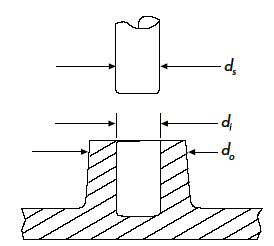
\includegraphics[width=0.5\textwidth]{img/analysis/thruster/pressfit.png}
	\caption{Pressfit Interference Diameters \cite{pressfit}}
	\label{fig:pressfit}
\end{figure}

\begin{equation}
n=\frac{S_y}{\sigma_r}=1.5
\end{equation}

\begin{equation}
{\sigma_r}=\frac{S_y}{n}=\frac{103MPa}{1.5}=68.67MPa
\end{equation}

\begin{equation}
\sigma_r=\frac{\delta}{R[\frac{1}{E_o}\cdot{}(\frac{r_o^2+R^2}{r_o^2-R^2}+v_o)+\frac{1}{E_i}\cdot{}(\frac{R^2+r_i^2}{R^2-r_i^2}+v_i)]}
\end{equation}	 
	
\begin{multline}
\delta = {68.67MPa}\cdot{}14.06mm[\cdot{}\frac{1}{68.9\cdot{10^3MPa}}\cdot{(\frac{(19.12mm)^2+(14.06mm)^2}{(19.12mm)^2-(14.06mm)^2}+0.33)}  
	\\ +\frac{1}{193\cdot{10^3MPa}}\cdot{(\frac{(14.06mm)^2+(12mm)^2}{(14.06mm)^2-(12mm)^2}-0.27)}]
\end{multline}

\begin{equation}
	\delta=0.082mm
\end{equation}
\\
Therefore, the bearing should be 0.082mm radially larger than the Bearing Bracket.
For the nylon 6 shaft in the bearing, a different pressfit calculation was used to calculate the same value (optimized for plastic \cite{pressfit}).

\begin{equation}
	n=\frac{S_y}{\sigma_r}
\end{equation}

\begin{equation}
{\sigma_r}=\frac{S_y}{n}=\frac{103MPa}{1.5}=68.67MPa
\end{equation}

\begin{equation}
i_a=(12mm)\cdot{}\frac{(68.67MPa)}{68.9\cdot{}10^3MPa}\cdot{}
\frac{(14mm)^2+(12mm)^2}{2(14mm)^2}=0.010mm
\end{equation}
\\
Therefore the shaft should be 0.01mm larger than the bearing inner diameter to provide an acceptable press fit.
\end{document}